\chapter{Arquitectura del sistema}
\section{Diseño general del sistema}
La aplicación de escritorio está construida con Electron, JavaScript, HTML y CSS. Para renderizar los documentos usa la biblioteca PDF.js, y para modificarlos (eliminar, reordenar y unir páginas) usa pdf-lib. Electron separa la aplicación en dos tipos de proceso, y esa separación estructura todo el diseño.

El proceso principal corre en Node.js. En él, main.js registra los canales de comunicación, elimina el menú predeterminado del sistema y crea la ventana principal. Desde este proceso se muestran los diálogos de abrir y guardar archivos, se construye el menú contextual nativo, se leen y escriben los archivos, se modifican los PDF y se conserva el estado de la aplicación.

El proceso renderer corre en Chromium. Es el que dibuja la interfaz, renderiza las páginas del documento, atiende el teclado y el mouse, y muestra los paneles, la búsqueda y los diálogos. Existe una segunda página, pdf-presentation-screen.html, que se abre en una ventana propia a pantalla completa para el modo presentación.

El código se organiza por responsabilidad, en directorios:

\begin{itemize}
  \item \verb|windows/|: crea y configura las ventanas (principal y de presentación) y el menú contextual.
  \item \verb|services/|: contiene la lógica de abrir, guardar, eliminar páginas, reordenar, anexar y el estado global
  \item \verb|ipc/|: es una capa que expone cada servicio mediante ipcMain.handle.
  \item \verb|renderer/|: contiene la interfaz, dividida por funcionalidad: visor, búsqueda, panel lateral, zoom, eliminación de páginas, ventana flotante y apertura y guardado.
\end{itemize}



 

El renderer se comunica con el proceso principal a través de \verb|preload.js|, que expone un único objeto, \verb|electronAPI|, con las operaciones permitidas (abrir, guardar, eliminar páginas, reordenar, leer y escribir el estado, etc.). Cuando el usuario elige una opción del menú contextual, el proceso principal envía un mensaje al renderer y este ejecuta la acción. El proyecto sigue un estándar de nombres, estructura de archivos, ramas y commits (Conventional Commits) documentado en \verb|docs/standard.md|.     

\begin{figure}[H]
	\centering
	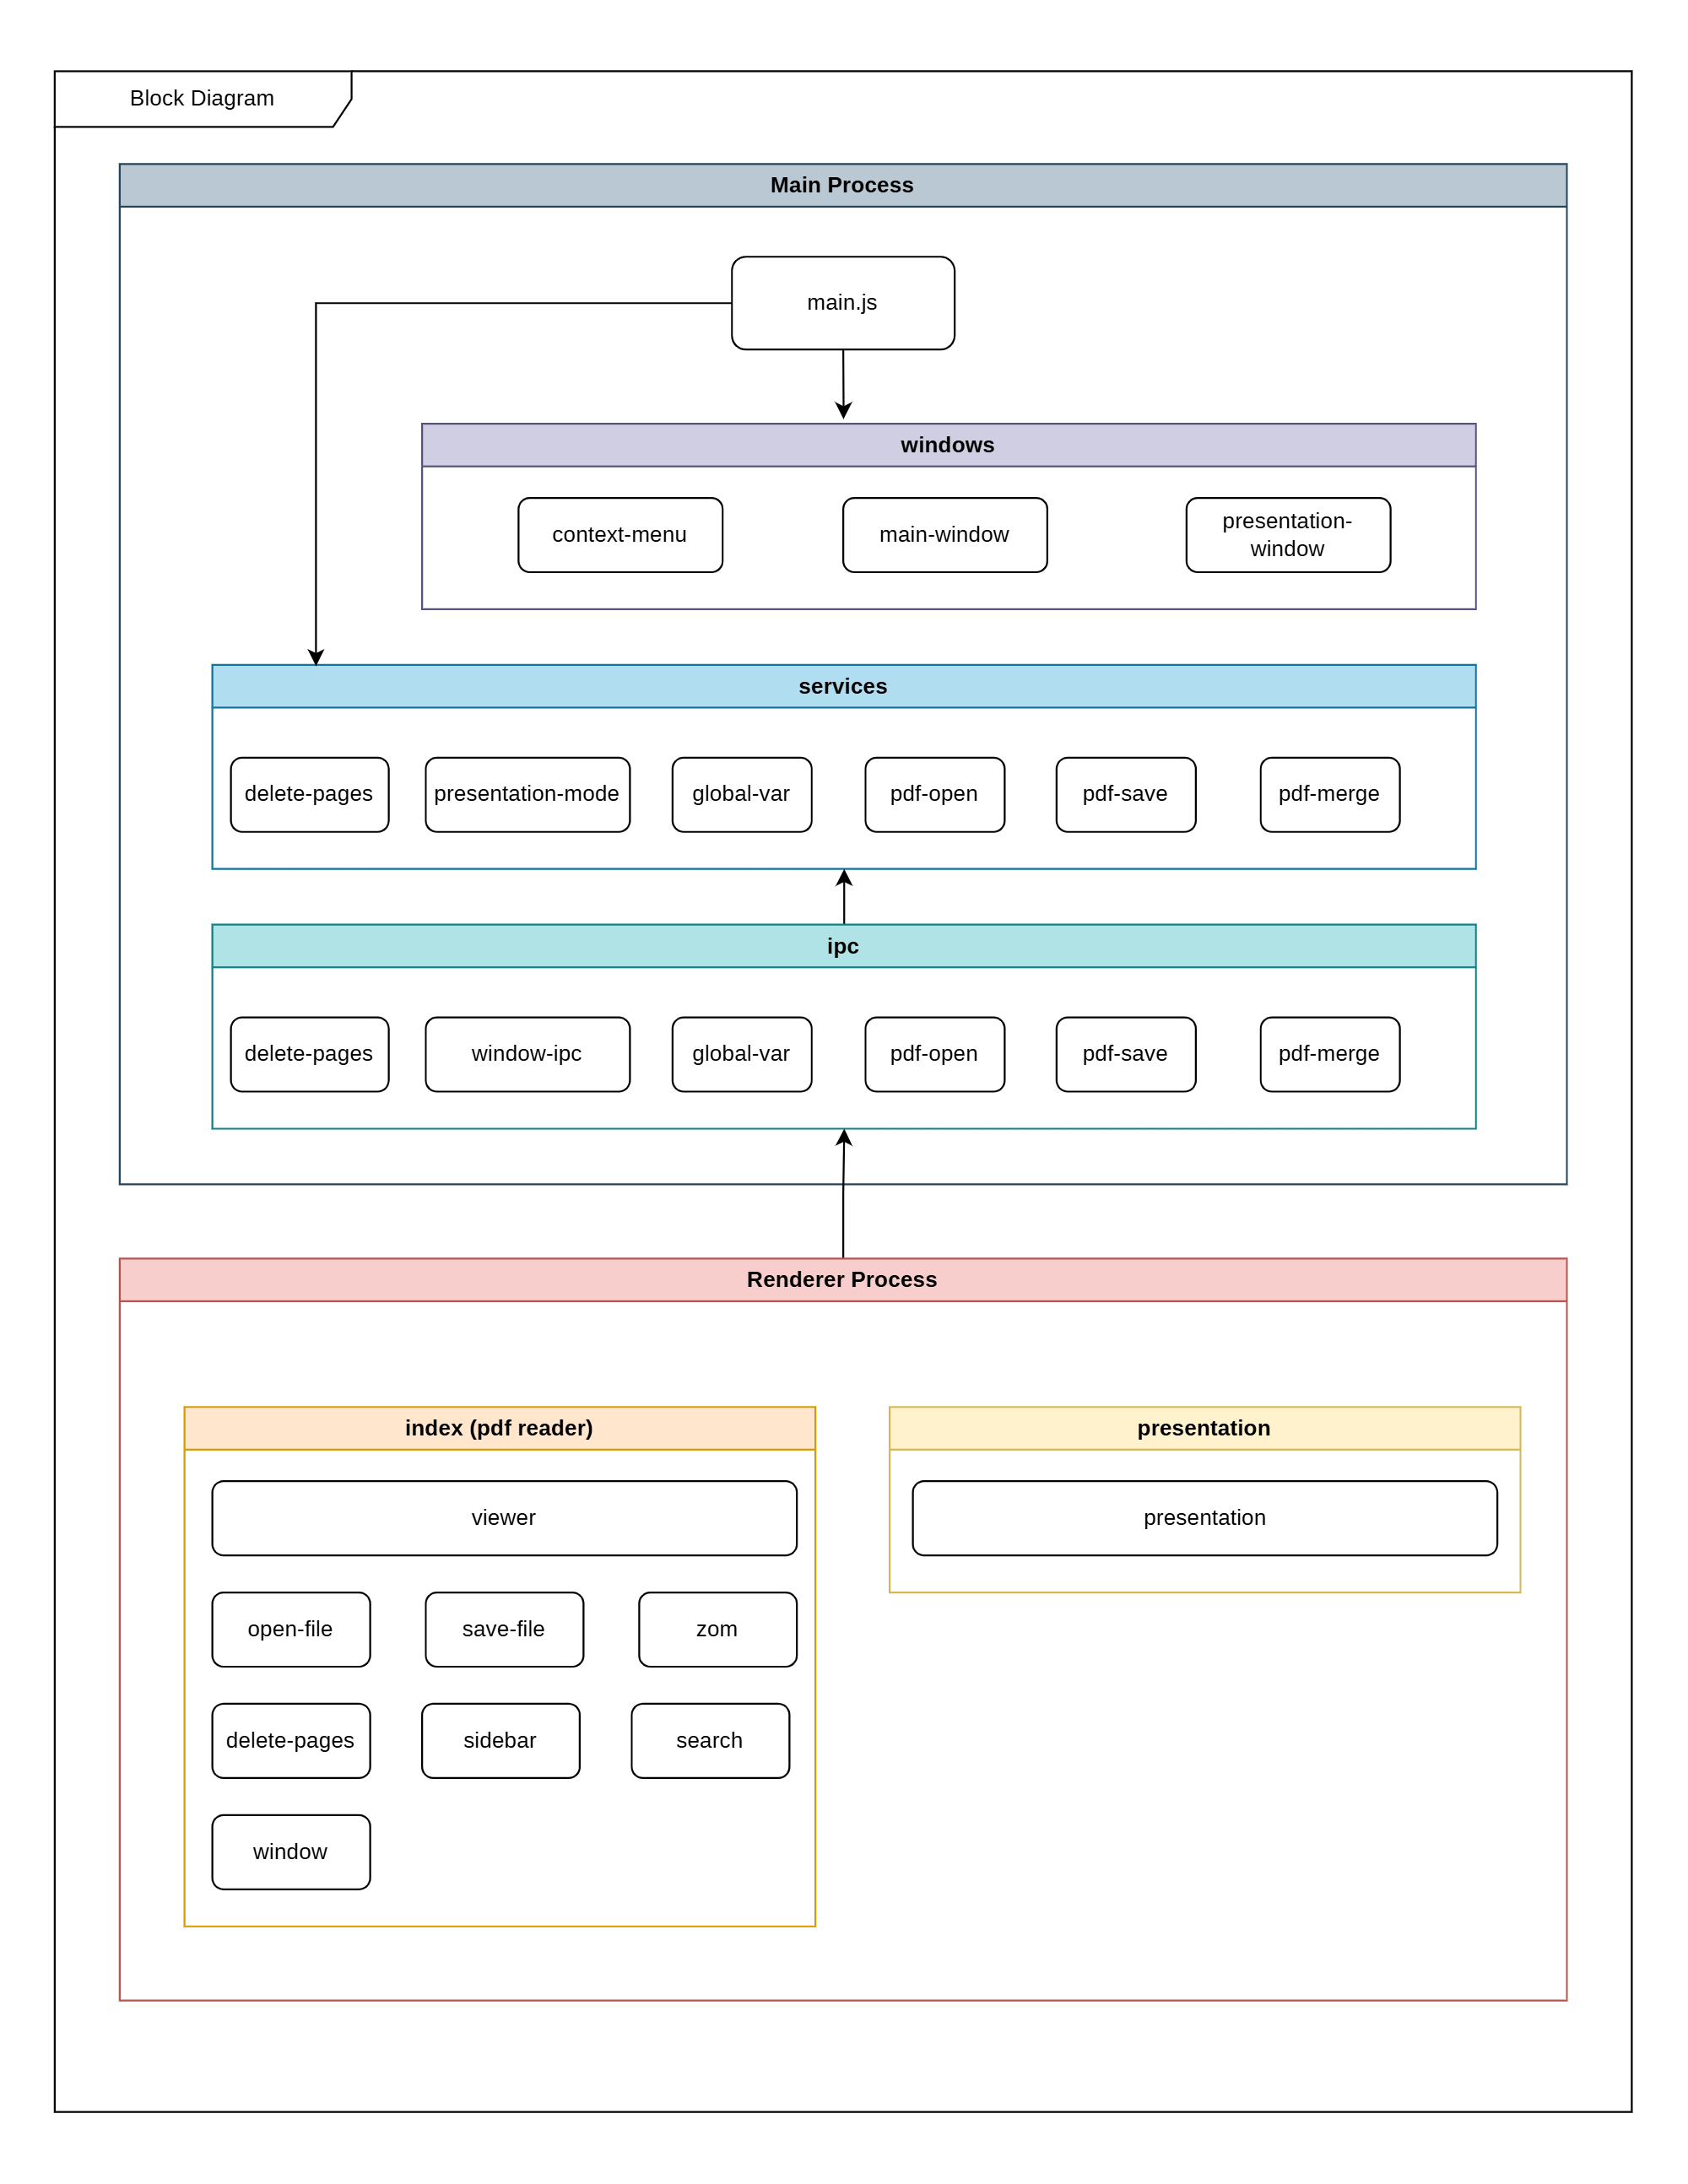
\includegraphics[width=\linewidth]{project/images/blockdiagram.png}
	\caption{\textbf{Diagrama de Bloques}}
	\label{DiagramaBloques}
\end{figure}


\subsection{Diseño de la persistencia}
El sistema no utiliza base de datos, por lo que no se elaboraron los modelos Entidad-Relación ni relacional. Un documento abierto se mantiene en memoria y solo se escribe en disco cuando el usuario ejecuta "Save" o "Save As". No se guarda ninguna otra información entre ejecuciones.

Mientras la aplicación está abierta, el estado vive en el proceso principal en tres variables: la ruta del archivo abierto, los bytes del documento con sus modificaciones y la página actual. El renderer las consulta al iniciar, porque su página se recarga después de cada operación de edición. La ventana de presentación las usa para mostrar el mismo documento. Las ediciones (eliminar páginas, reordenar y anexar) reemplazan esos bytes con el PDF modificado.

\subsection{Diagrama de clases}
%Añada una imagen con el diagrama de clases del sistema,  preferiblemente desarrollado en DIA. Introdúzcala con un párrafo breve que enlace el diagrama con la descripción en prosa del encabezado de sección. Se recomienda que el diagrama se diseñe de forma que calce bien en una página vertical, de forma que se facilite su lectura. Recuerde hacer referencia a su diagrama de clases usando la referencia correcta. Por ejemplo, en la Figura \ref{DiagramaClases} se encuentra el diagrama de clases.
% \begin{figure}[H]
%  \centering
%    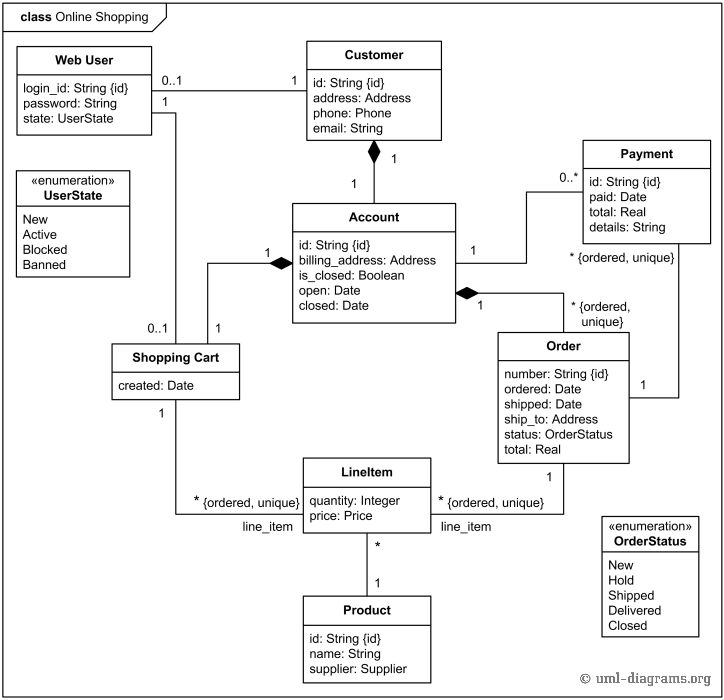
\includegraphics[ width=15cm]{project/images/class-example-online-shopping-domain.png}
%  \caption{\textbf{IMAGE CAPTION}}
%  \label{DiagramaClases}
% \end{figure}
La Figura \ref{DiagramaClases} muestra las dos clases que estructuran el visor. Son las únicas clases del sistema que mantienen estado propio. El resto de la lógica está en módulos de funciones, como el zoom, la búsqueda, el panel lateral y las operaciones de edición. Ambas clases reciben los bytes del documento, que obtienen del proceso principal, y los abren con PDF.js. No hay herencia ni relación directa entre ellas, porque cada una se usa en una página distinta: \verb|PdfViewer| en la ventana principal y \verb|PdfPresentationViewer| en la ventana de presentación.

PdfViewer es el visor de lectura continua. Mantiene los bytes del documento (\verb|dataPDF|), el documento abierto (\verb|documentPDF|), la página actual y la anterior (\verb|currentPage|, \verb|previousPage|), el estado del zoom (\verb|zoomState|) y el conjunto de páginas del documento (\verb|pages|), donde guarda para cada una su contenedor, su lienzo y si está dibujada. Tiene también tres atributos de retrollamada (\verb|onTextLayerRendered|, \verb|onTextLayerUnloaded| y \verb|onCurrentPageChanged|), con los que avisa a otros módulos. Por ejemplo, el módulo de búsqueda los usa para actualizar los resaltados y el panel lateral para marcar la miniatura de la página actual. Sus métodos se agrupan en:

\begin{itemize}
    \item \textbf{Carga y dibujo:} \verb|load()| abre el documento y \verb|renderPages()| crea, para cada página, el contenedor con su lienzo y su capa de texto seleccionable. Las páginas solo se dibujan cuando se acercan a la pantalla y se liberan cuando se alejan, lo que mantiene bajo el consumo de memoria.
    \item \textbf{Navegación:} \verb|updateCurrentPage()| determina qué página está en el centro de la ventana y actualiza el contador. \verb|skipUp()| y \verb|skipDown()| mueven a la página anterior o siguiente, \verb|jumpToPage()| salta a una página y \verb|jumpToPagePosition()| salta a un punto exacto de una página, que es lo que usa el outline.
    \item \textbf{Zoom y ajuste:} \verb|zoomAtPoint()| acerca o aleja manteniendo fijo el punto bajo el cursor, \verb|resetZoom()| regresa al 100 \% y \verb|fitWidth()| ajusta el documento al ancho de la ventana, que usa la ventana flotante.
\end{itemize}

PdfPresentationViewer es el visor del modo presentación. Muestra una sola página a la vez sobre un único lienzo (\verb|canvas| y \verb|context|), ajustada al tamaño de la pantalla (\verb|scale|), y arranca en la página que el usuario estaba leyendo (\verb|currentPage|). Sus métodos son \verb|load()|, que abre el documento; \verb|nextPage()| y \verb|prevPage()|, que cambian de página; y \verb|renderPage()|, que la dibuja. Los atributos \verb|pageIsRendering| y \verb|pageNumberIsPending| junto con \verb|queueRenderPage()| evitan que se superpongan dos dibujados: si se pide otra página mientras una se está dibujando, la solicitud queda pendiente y se atiende al terminar.

 



 \begin{figure}[H]
  \centering
    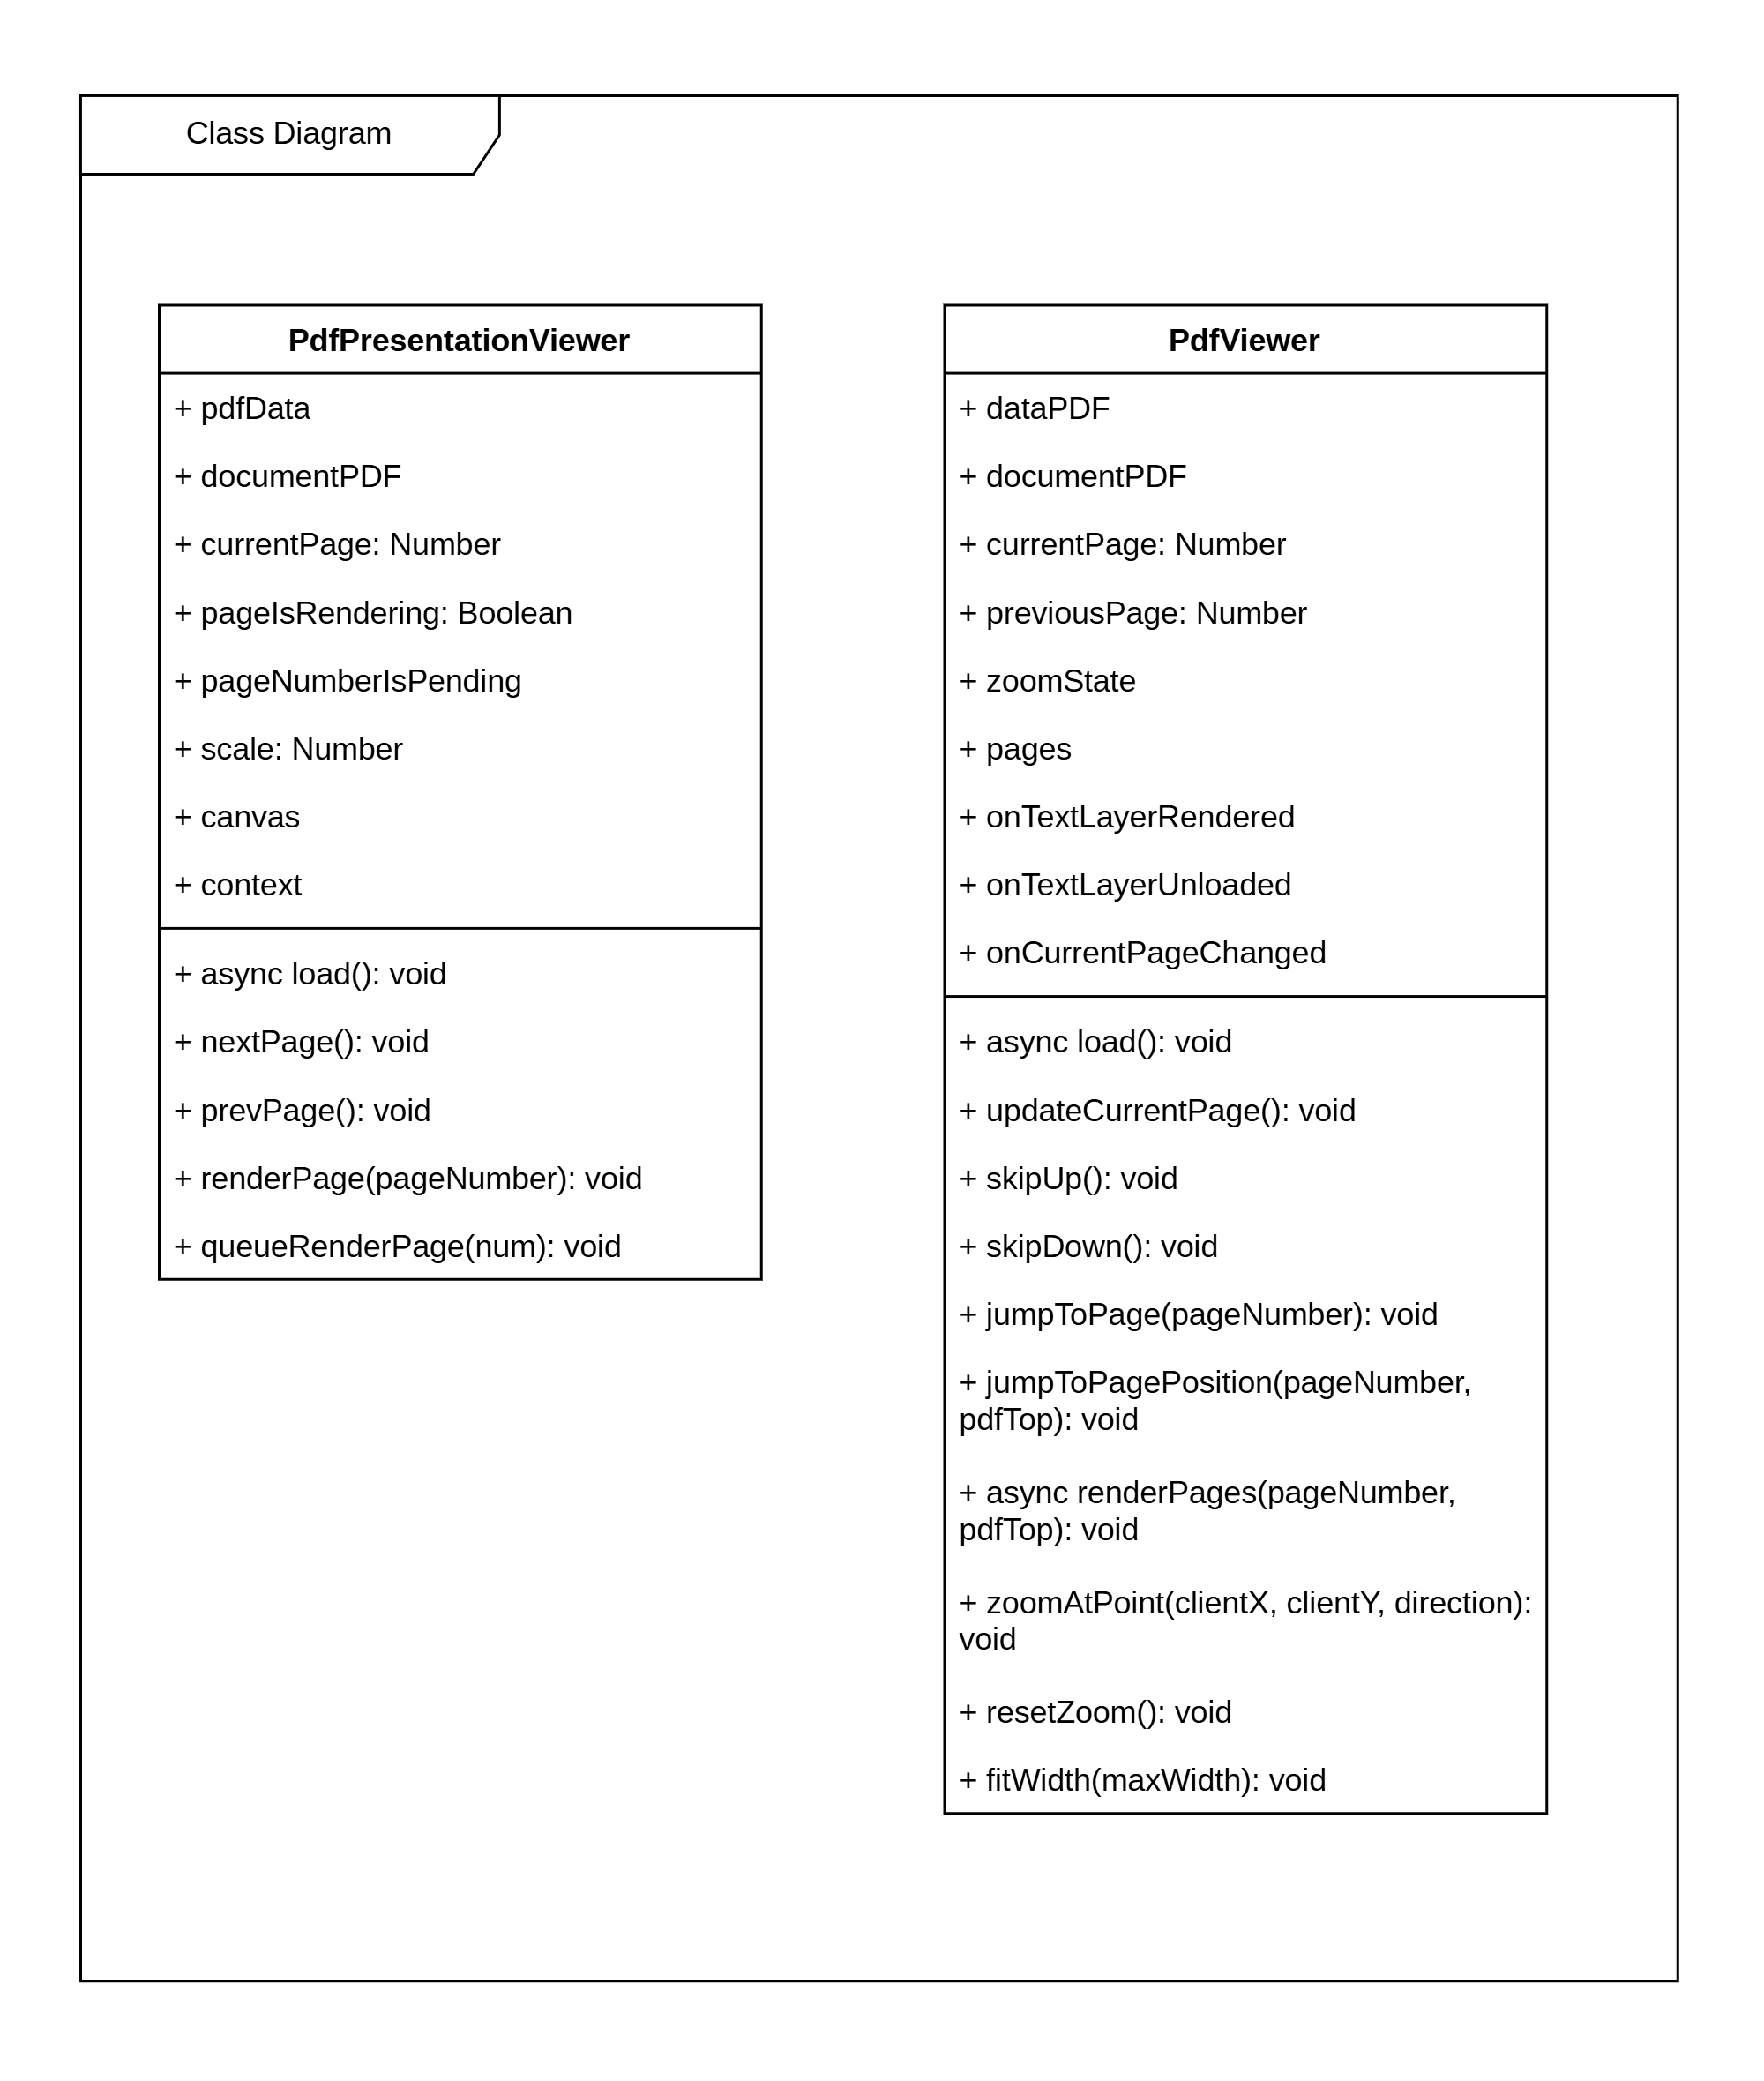
\includegraphics[ width=15cm]{project/images/classdiagram.png}
  \caption{\textbf{Diagrama de Clases}}
  \label{DiagramaClases}
\end{figure}

